\subsection{Верификация создаваемого проекта}
Важнейшим этапом проектирования электронного устройста является выполнение
верификации созданных принципиальной электрической схемы и печатной платы.
Этот процесс выполняется средствами используемой EDA системы
для того, чтобы проверить удовлетворяет ли спроектированное устройство набору
конкретных требований.

Процесс физической верификации включает в себя:
\begin{itemize}
	\item{} контроль геометрических проектных норм (DRC);
	\item{} контроль электрических проектных норм (ERC);
	\item{} сравнение топологической схемы с исходной (LVS);
	\item{} выполнение проверки антенных эффектов.
\end{itemize}


\subsubsection{Контроль геометрических проектных норм}
Контроль геометрических проектных норм позволяет проверить удовлетворяют ли физические
размеры конкретной печатной платы и расположенные на ней компоненты, контактные
площадки и корпуса устройств, требованиям конкретного производителя печатных плат.
Производителем такие требования формируются на основе ограничений, исользуемого для
производства печатных плат оборудования.

Программа контроля проектных норм в системе Eagle работает непосредственно с топологией.
Контроль осуществляется автоматически по значениям конструкторско--технологических
требований (DRC--контроль), заранее полученным в файле конфигурации от производителя
печатных плат, либо введённые вручную при первом выполнении контроля.

Любые выходы за рамки ограничений помечаются непосредственно на изображении топологии,
выводимом на экран дисплея.

Запукс программы контроля правил проектиирования в системе Eagle осуществляется из
редактора топологической схемы командой ''DRC''.  При вводе этой команды на экран
выводится диалоговое окно задания параметров проверки (рис. \ref{img:drc}).
\begin{figure}[ht]
	\center{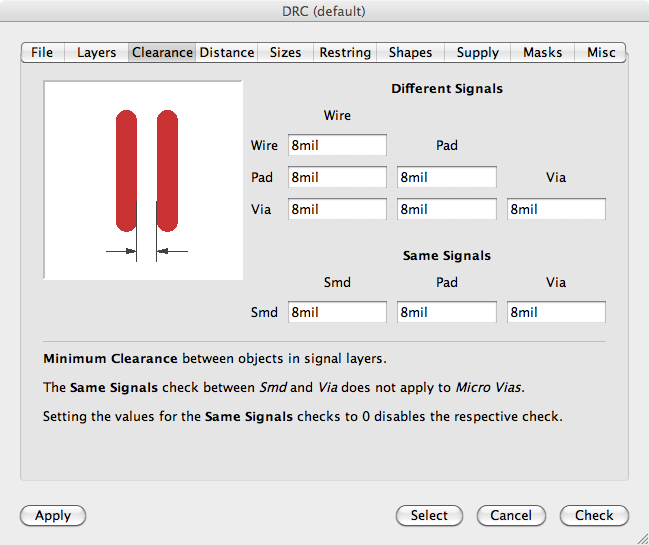
\includegraphics[bb=0 0 649 545, clip, scale=0.5]{drc.png}}
	\caption{Диалоговое окно программы контроля правил проектирования системы Eagle}
	\label{img:drc}
\end{figure}

DRC-контроль системы Eagle позволяет провести контроль следующих параметров:
\begin{itemize}
	\item{} контроль просветов -- проверяет на соотвествие правилам расстояния между
		проводниками и контактными площадками;
	\item{} контроль расстояний -- проверяет расстояние между сигнальными
		линиями и границами печатной платы;
	\item{} контроль размеров -- проверяет размеры объектов расположенных в сигнальном
		слое (таких как отверстия и контактные площадки).
\end{itemize}

\subsubsection{Контроль электрических проектных норм}
В результате проведения этой проверки идентифицируются все нераспознанные или
неправильно соединенные элементы, а также все нарушения электрических проектных норм.

В системе Eagle, ERC проверка выявляет несоответствия между линиями питания и общим проводом,
несоответствия соединений конкретным сигналам, включая проверку по типам выводов.
При проведении этого вида контроля Eagle так же выполняет сравнение топологической схемы
с принципиальной (Consistency Check).

\begin{figure}[ht]
	\center{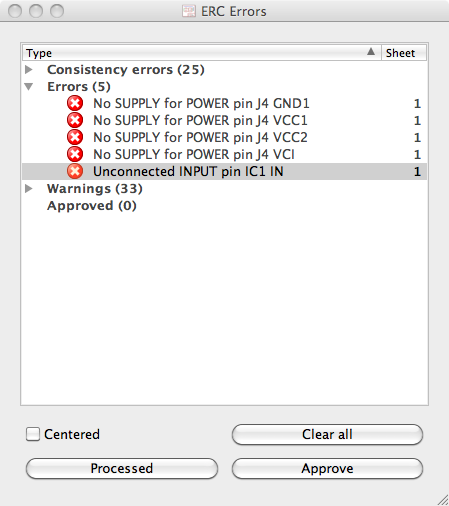
\includegraphics[bb=0 0 449 506, clip, scale=0.5]{erc.png}}
	\caption{Диалоговое окно списка ошибок выявленных контролем электрических проектных норм}
	\label{img:erc}
\end{figure}

Для выполнения этой проверки необходимо в редакторе принципиальных схем (Eagle Layout Editor)
выполнить команду ''ERC''. В случае обнаружения ошибок, на экран будет выведено диалоговое окно
со списком ошибок (рис. \ref{img:erc}). Нажание на элемент отображённых в списке ошибок приводит
к тому, что Eagle подсвечивает место предполагаемой ошибки.


\subsubsection{Проверка антенных эффектов}
Антенный эффект --  явление излучения или приема радиоволн, не предназначенными для этого
предметами.

Бесплатная версия Eagle не имеет инструментов проверки антенных эффектов. Однако, так как
полностью избавиться от них невозможно \cite{antennaeff}, проектируемое устройство работает
на относительно низкой частоте, а антенный эффект сетевого модуля нивелируется конструкцией
коннектора MagicJack, то такая проверка является избыточной, вследствии чего
она не производилась.
